% =======================================================================
\section{Methods}

\subsection{Data}
\label{sec:data}

The primary single-match analysis uses SkillCorner open broadcast
tracking data \citep{SkillCorner2024}, match ID 1996435 (Sydney FC
versus Adelaide United, A-League 2024/25). Positions are recorded at
10 frames per second as $(x, y)$ coordinates in metres on a standard
football pitch model. Only frames with complete 22-player coverage are
retained, which yields 43{,}531 frames (approximately 72 minutes at
this sampling rate). The multi-match sample comprises that match and
nine further A-League matches from the same repository. Each match
contributes approximately 39{,}000--49{,}000 complete frames, and the
ten matches together give 436{,}648 frames. SkillCorner match IDs and
fixtures are listed in Supplementary Table~\ref{tab:matches}.

Consecutive complete frames share nearly the same configuration, so
the full stream is not treated as a sequence of independent snapshots.
Prevalence and organisational-level summaries are estimated on a
uniform subsample instead. Write $t$ for the time of a complete frame
in the native stream. The same operational rule is used on every
match: list the complete 22-player frames, set the stride to
$\lfloor N/150\rfloor$, and retain 150 frames. Write $\tilde{t}$ for a
time retained by that rule, and $\tilde{T}$ for the set of such times
on one match, so $|\tilde{T}|=150$. On the primary match
$N = 43{,}531$, so the stride is 290 frames ($\approx 29$~s). Across
ten matches the sampled times give 1{,}500 frames.

This subsample limits temporal pseudo-replication. It does not treat
the competitive-dependence inference problem named in
Section~\ref{sec:background}, and it cannot resolve formation or
dispersion of loops between samples. Event association is a
construct-validity check, not a dynamical model, and it does not use
$\tilde{T}$. Topology for that check is computed on every tenth
complete frame (1~Hz). Supplementary Figure~\ref{fig:acf} records the
autocorrelation of those 1~Hz summaries on the primary match, as a
diagnostic. The figure does not determine the subsample
$\tilde{T}$.

\subsection{Hierarchical clustering}
\label{sec:clustering}

On this corpus the named organisational levels of
Section~\ref{sec:scaleconflation} (individual, small group, envelope)
are instantiated as individual, tactical, and team. The class names
those levels by cardinality. The cutoffs $\delta$ that select them are
therefore read from the sweep in
Section~\ref{sec:cutoffselection}, rather than assumed in metres.

Figure~\ref{fig:pipeline} summarises the pipeline of
Sections~\ref{sec:clustering}--\ref{sec:cycles}. The pipeline is
applied at the sampled times $\tilde{t}\in\tilde{T}$ of
Section~\ref{sec:data}. The input is the point cloud
$P(\tilde{t}) = \{p_1(\tilde{t}), \dots, p_{22}(\tilde{t})\}
\subset \mathbb{R}^2$.

\begin{figure}[t]
\centering
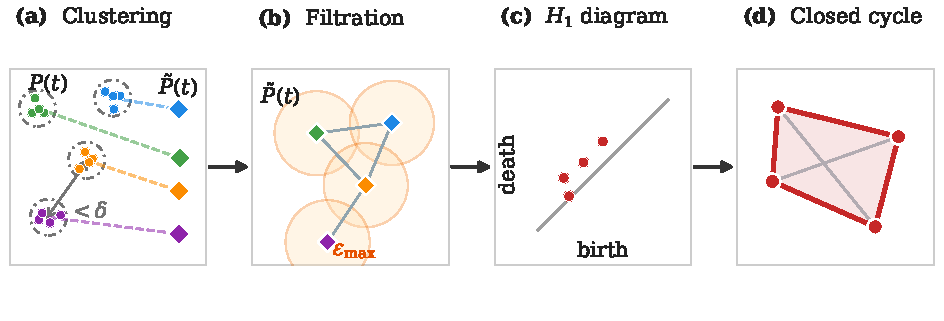
\includegraphics[width=\textwidth]{figures/fig1_pipeline_schematic}
\caption{Analysis pipeline on a bounded domain (schematic geometry on
a football pitch; each panel shows the step and its output).
\textbf{(a)}~Colour-coded local groups in
\texorpdfstring{$P(\tilde{t})$}{}
with dashed \texorpdfstring{$\delta$}{}-disks and a representative
gap \texorpdfstring{$<\delta$}{} (Section~2.2).
\textbf{(b)}--\textbf{(d)}~Vietoris--Rips (VR) on the cluster centroids
\texorpdfstring{$\tilde{P}(\tilde{t})$}{} at three increasing
\texorpdfstring{$\varepsilon$}{}, truncated at
\texorpdfstring{$\varepsilon_{\max}$}{}
(equation~\eqref{eq:adaptive}; Section~2.4).
\textbf{(e)}~Finite \texorpdfstring{$H_1$}{} birth--death pairs.
\textbf{(f)}~The same pairs as a barcode.
\textbf{(g)}~Graph-cycle proxy for an \texorpdfstring{$H_1$}{} pair
(Section~2.5). Figure~\ref{fig:cycles} shows the cycle step on real
tracking data.}
\label{fig:pipeline}
\end{figure}

Single-linkage hierarchical clustering is applied at a cutoff
distance $\delta > 0$. It partitions $P(\tilde{t})$ into clusters
$C_1, \dots, C_k$ in which every pair of points is connected by a
chain of pairwise distances not exceeding $\delta$. Each cluster is
replaced by its centroid, giving the reduced point cloud
\[
\tilde{P}(\tilde{t})=\left\{\bar{c}_j : \bar{c}_j=\frac{1}{|C_j|}\sum_{p\in C_j} p,\ j=1,\dots,k\right\},
\]
and persistent homology is then computed on $\tilde{P}(\tilde{t})$
rather than on $P(\tilde{t})$.

Complete-linkage and Ward's method are not used for the headline
analysis. Their effect on $H_1$ counts is examined in
Section~\ref{sec:limitations}. Team identity is withheld as an input,
so the partitions are spatial rather than labelled by side.

\subsection{Cutoff selection}
\label{sec:cutoffselection}

The class names the three organisational levels by cardinality. The
selector therefore inverts a named cluster count rather than assuming
a length in metres. The inversion is read from the pooled mean
cluster-count curve on this corpus.

A complete frame has $n=22$ agents. The sweep uses every complete
22-player frame of the ten matches in Supplementary
Table~\ref{tab:matches} (436{,}648 frames). The grid is
$\delta\in[0.25, 40.0]$~m at $0.25$~m steps (160 points). No random
window is drawn, and epoch lengths are not mixed. Clustering is
single-linkage, and team labels are unused.

Let $\overline{H_0}(\delta)$ be the mean cluster count at cutoff
$\delta$, pooled over those frames. Let $P(k\ge 4;\delta)$ be the
fraction of frames with at least four clusters. The three inversion
rules are then as follows:

\begin{itemize}
\item individual: largest $\delta$ with $\overline{H_0}(\delta)\ge n-3=19$;
\item tactical: $\delta$ minimising
$|\overline{H_0}(\delta)-5|$, among candidates with
$P(k\ge 4;\delta)\ge 0.5$;
\item team: smallest $\delta$ with $\overline{H_0}(\delta)\le 2$.
\end{itemize}
Ties take the smaller $\delta$. The three targets are roster
statements. The individual target $n-3=19$ is a mostly resolved set of
agents. The tactical target $5$, with $k\ge 4$ still common, is a
handful of coordinating groups that remain loop-feasible. The team
target $2$ is at most two spatial envelopes.

On this corpus the inversion returns $2.75$~m, $11.75$~m, and
$23.0$~m. Pooled mean $H_0$ at those cutoffs is $19.31$, $5.06$, and
$1.98$. Inverting each match separately gives
$2.80\pm 0.20$~m, $11.80\pm 0.35$~m, and $22.98\pm 0.72$~m
(mean $\pm$ s.d.\ across matches). Acceptance requires every match's
mean $H_0$ at the pooled cutoff to lie in $[15, 22]$, $[4, 10]$, and
$[1, 2.5]$ respectively. All ten matches lie inside those bands.

The curve is asymmetric. Micro-structure merges quickly, at about
$1.6$ clusters per metre from $\overline{H_0}=19$ to $5$.
Macro-structure then resists merging, at about $0.27$ clusters per
metre from $5$ to $2$. The remaining gaps are the large between-group
distances. That flattening is why the team cutoff sits far out at
$23.0$~m and still returns two envelopes, not two teams.

Clustering-quality diagnostics (Calinski--Harabasz, silhouette, and
Shannon entropy of cluster sizes) are recorded on a deterministic
1~Hz subset (every 10th complete frame). Silhouette is omitted when
$k=1$; it is not coded as 0. Those curves are alternatives, not
adopted cutoffs, and are reported in Supplementary
Figure~\ref{fig:diagnostics}. Figure~\ref{fig:cutoff} shows the
estimator and its spatial realisation.
Section~\ref{sec:sensitivity} reports how tactical $H_1$ detection
responds to the cutoff choice.

\begin{figure}[t]
\centering
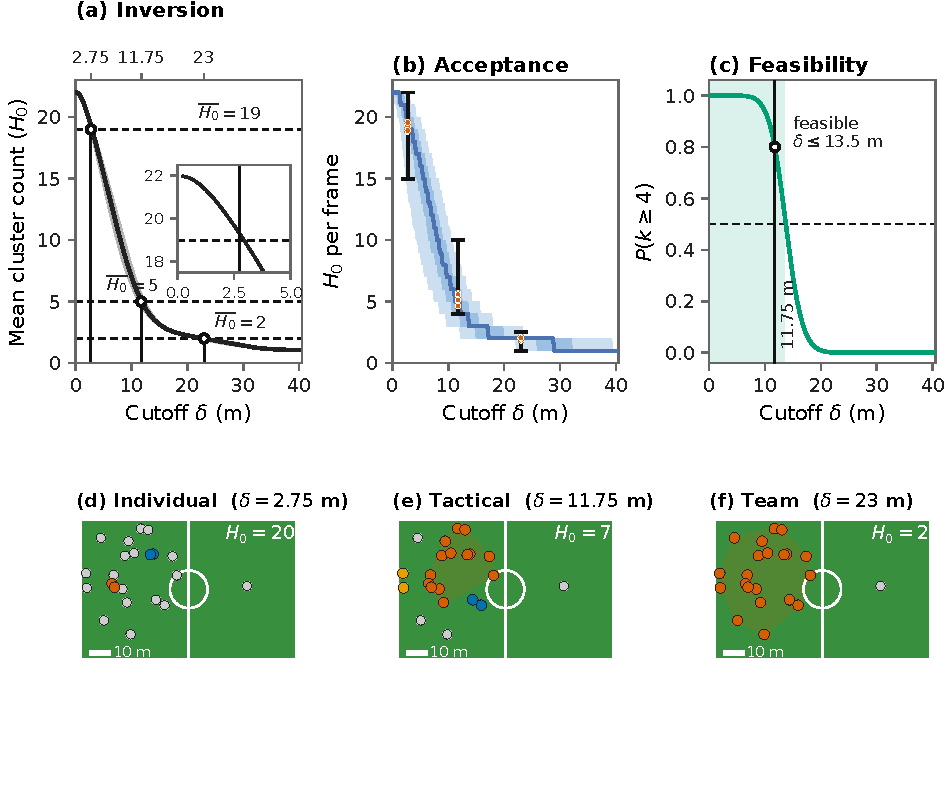
\includegraphics[width=\textwidth]{figures/fig2_cutoff_sweep}
\caption{Cutoff selection by cardinality inversion. Sweep on all
complete frames of the ten SkillCorner matches (436{,}648 frames);
not the 150-frame sample \texorpdfstring{$\tilde{T}$}{} of
Section~\ref{sec:data}. Grid
\texorpdfstring{$\delta\in[0.25, 40.0]$}{}~m at $0.25$~m.
\textbf{(a)}~Pooled mean cluster count
\texorpdfstring{$\overline{H_0}(\delta)$}{} (black) with the ten
per-match curves (grey). Targets are roster statements:
\texorpdfstring{$\overline{H_0}=n-3=19$}{} (most agents resolved),
\texorpdfstring{$\overline{H_0}=5$}{} (a few coordinating groups,
loop-feasible), and \texorpdfstring{$\overline{H_0}=2$}{} (two spatial
envelopes, not the two teams, since team labels are unused). Circles
mark the inversion at $2.75$, $11.75$, and $23.0$~m (top axis); the
inset zooms the individual rule.
\textbf{(b)}~Per-frame \texorpdfstring{$H_0$}{} distribution (median,
interquartile band, and 5th--95th centile band). Vertical brackets are
the acceptance intervals \texorpdfstring{$[15,22]$}{},
\texorpdfstring{$[4,10]$}{}, and \texorpdfstring{$[1,2.5]$}{}; orange
dots are the ten per-match means, all inside. Frame-to-frame variance
is why the acceptance intervals, not a single per-frame count, define
the test.
\textbf{(c)}~Feasibility of the tactical rule.
\texorpdfstring{$k$}{} is the number of clusters in a frame and
\texorpdfstring{$P(k\ge 4)$}{} the fraction of frames with at least
four; the adopted $11.75$~m sits at \texorpdfstring{$P=0.80$}{}, inside
the feasible region (\texorpdfstring{$\delta\le 13.5$}{}~m).
\textbf{(d--f)}~The same cutoffs on primary-match sample frame~95
(\texorpdfstring{$H_0=20,7,2$}{}; one frame, near the pooled targets
$19$, $5$, $2$). Coloured hulls are multi-player clusters, grey are
singletons; colours distinguish separate topological components in this
frame, not player teams. Each pitch carries a $10$~m scale bar.
Clustering-quality diagnostics are in Supplementary
Figure~\ref{fig:diagnostics} and are not the selector.}
\label{fig:cutoff}
\end{figure}

\subsection{Maximum filtration distance}
\label{sec:adaptivefiltration}

Clustering at cutoff $\delta$ produces a reduced point cloud
$\tilde{P}(\tilde{t})$. Inter-centroid distances on that cloud are typically
larger than $\delta$. A maximum filtration distance
$\varepsilon_{\max}$ fitted to one cutoff can then return no $H_1$ at
another.

The Vietoris--Rips complex itself is not modified. Its parameter is
truncated at
\begin{equation}
\varepsilon_{\max} = \max\Big(P_{75}\{d(\bar c_i,\bar c_j) : i<j\},\; \max(5.0,\,2\delta)\Big).
\label{eq:adaptive}
\end{equation}
Here $P_{75}$ is the 75th percentile of pairwise inter-centroid
distances on $\tilde{P}(\tilde{t})$. The first term tracks the geometry of the
reduced cloud at the current cutoff. The second term is a floor that
prevents a degenerate filtration at small $\delta$. The same floor
keeps the filtration in the inter-cluster distance regime.

$P_{75}$ is a conventional upper-quartile summary.
Section~\ref{sec:sensitivity} reports an ablation across $P_{50}$
through $P_{95}$. Every tested percentile returns identical $H_1$
totals and frame-presence rates. The choice is therefore a reporting
convention, not an optimisation.

Persistence diagrams are computed with Ripser via Ripser.py
\citep{bauer2021ripser}, with coefficients in $\mathbb{F}_2$. We report
finite $H_1$ bars. The Results use three summaries of those bars. None
of them is a duration in seconds. \emph{Presence} is the fraction of
frames with at least one finite $H_1$ bar. \emph{Filtration lifetime}
$p$ is death minus birth, in metres on the Vietoris--Rips parameter:
the length of a bar, not a duration in seconds. \emph{Total
persistence} is the sum of $p$ over the finite bars in a frame. It is
the Spearman input in Section~\ref{sec:complementarity}. The 150-frame
subsample of Section~\ref{sec:data} does not measure how long a loop
lasts on the clock. The $H_0$ counts reported in
Section~\ref{sec:scaleh0} are read from these diagrams at filtration
zero. We cross-checked all
primary-match diagrams against GUDHI \citep{gudhi2014} and giotto-tda
\citep{tauzin2021}. Birth--death pairs agreed to within numerical
tolerance ($10^{-6}$~m). GUDHI is also used for the bottleneck-distance
and landscape computations reported in
Section~\ref{sec:complementarity}.

\subsection{Closed cycle identification}
\label{sec:cycles}

Each $H_1$ feature corresponds to a 1-cycle in the Vietoris--Rips
complex. A geometric realisation is recovered from the adjacency graph
of edges whose distances fall within the feature's persistence
interval $[\text{birth},\text{death}]$. Closed cycles of length at
least 3 are then enumerated by breadth-first search from each vertex.
If that graph yields no cycle, the search falls back to edges with
length in $[\tfrac{1}{2}\text{birth},\,\text{death}]$. Breadth-first
search is used in preference to depth-first search because it
prioritises shorter cycles. Those shorter cycles correspond to minimal
enclosing arrangements. Among the enumerated cycles, the
representative is the one whose edge distances lie closest to the
midpoint of the persistence interval. This representative is a
geometric proxy for the persistence pair, not a homology generator
extracted from the matrix reduction.

\subsection{Statistical tests}
\label{sec:stats}

$H_1$ detection could reflect the number of centroids rather than
their arrangement. Each frame is therefore compared against a matched
null. For a frame whose clustering yields $k$ centroids, the null
draws $k$ points uniformly from the convex hull of those same
centroids. Cardinality and spatial envelope are thus held fixed. Only
the arrangement is randomised. The truncation of
equation~\eqref{eq:adaptive} is recomputed on each null cloud.
Nothing else differs between the observed cloud and the null. We use
200 null replicates per frame. The reported statistic is the excess of
observed over null $H_1$ presence, with 95\% confidence intervals from
bootstrap resampling over matches.

Complementarity of the two $H_1$ levels
(Section~\ref{sec:complementarity}) is assessed by two frame-level
tests. The Spearman rank correlation is computed on total $H_1$
persistence: the sum of death minus birth over all finite $H_1$ bars in
a frame. The same correlation is also reported on loop counts, as a
robustness check. Fisher's exact test is computed on the binary
co-occurrence of $H_1$ presence at the two levels. Both statistics
carry 95\% confidence intervals obtained by bootstrap resampling over
matches (1{,}000 resamples), with the match as the resampling unit.
Bottleneck and landscape distances between the two levels' persistence
diagrams are computed using GUDHI, as described in
Section~\ref{sec:adaptivefiltration}.

The construct-validity check in Section~\ref{sec:eventcorr} uses a
Mann--Whitney test of $\Delta$ against zero.
Topology is evaluated on every tenth complete frame (1~Hz), not on
$\tilde{T}$. For each annotated event, $\Delta$ is the change in mean
total persistence from the five 1~Hz frames immediately before the
event to the five immediately after it. That window is five seconds
either side of the event; the event frame itself is excluded.
Event classes are pre-specified, and the $p$-values are nominal.

\subsection{Software and reproducibility}

All analyses were performed in Python~3.11. Persistence diagrams are
computed with Ripser.py~0.6.12 \citep{bauer2021ripser,tralie2018}.
Bottleneck distances and landscape representations use
GUDHI~3.11.0 \citep{gudhi2014}. giotto-tda~0.6.0 \citep{tauzin2021}
provided independent cross-checks. Supporting scientific Python packages
match the pinned \texttt{requirements.txt} accompanying the manuscript:
NumPy~2.0.2, SciPy~1.13.1, pandas~2.3.2, scikit-learn~1.6.1. Analysis
code, pipeline configuration, and pinned dependencies are included with
the manuscript materials. They will be released in a public repository
at arXiv posting (see Data Availability Statement).
